% Based on 
% http://tex.stackexchange.com/questions/15088/bipartite-graphs

\documentclass[12pt]{standalone}
\usepackage[rgb]{xcolor}
\definecolor{color1}{RGB}{0,114,178}
\definecolor{color2}{RGB}{0,158,115}
\definecolor{color3}{RGB}{213,94,0}

\usepackage{tikz}
\usetikzlibrary{chains,arrows}

\begin{document}

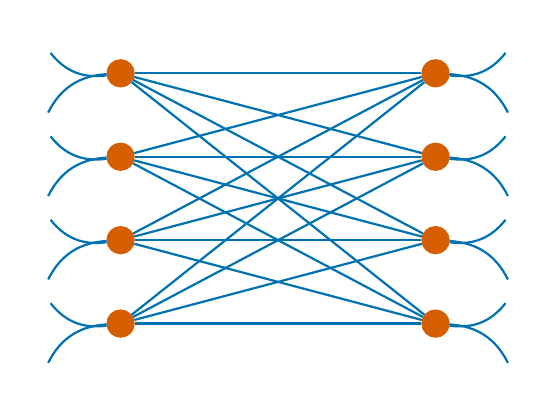
\begin{tikzpicture}[thick,
  leftnode/.style={circle,draw=color3,fill=color3},
  rightnode/.style={circle,draw=color3,fill=color3},
  blindnode/.style={draw=white,circle,fill=white}
]

% blind nodes
\begin{scope}[xshift=-1cm, yshift=4mm, start chain=going below,node distance=7mm]
\foreach \i in {1,2,...,5}
    \node[blindnode,on chain] (bl\i) [] {};
\end{scope}
\begin{scope}[xshift=5cm, yshift=4mm, start chain=going below,node distance=7mm]
\foreach \i in {1,2,...,5}
    \node[blindnode,on chain] (br\i) [] {};
\end{scope}


% the vertices of U
\begin{scope}[start chain=going below,node distance=7mm]
\foreach \i in {1,2,...,4}
    \node[leftnode,on chain] (l\i) [] {};
\end{scope}

% the vertices of V
\begin{scope}[xshift=4cm,start chain=going below,node distance=7mm]
\foreach \i in {1,2,...,4}
    \node[rightnode,on chain] (r\i) [] {};
\end{scope}

% the internal edges
\foreach \i in {1,2,...,4}
    \foreach \j in {1,2,...,4}
        \draw[color1] (l\i) -- (r\j);

% the external edges
\foreach \i in {1,2,...,4} {
    \path[color1] (l\i) edge [bend left] node {} (bl\i) ;
    \pgfmathtruncatemacro{\j}{\i + 1}%    
    \path[color1] (l\i) edge [bend right] node {} (bl\j) ;
}
\foreach \i in {1,2,...,4} {
    \path[color1] (r\i) edge [bend right] node {} (br\i) ;
    \pgfmathtruncatemacro{\j}{\i + 1}%    
    \path[color1] (r\i) edge [bend left] node {} (br\j) ;
}

\end{tikzpicture}
\end{document}
